\begin{figure}[t!]
    \centering
    \begin{minipage}{0.52\textwidth}
        \centering
        \captionof{table}{Quantitative ablation study for our proposed RL rewards in \ours{} on SimplerEnv, EgoPlan-Bench2, and RoboVQA benchmarks.}
        \resizebox{1.0\linewidth}{!}{
            \label{tab:ablation_reward}
            \begin{tabular}{lccccc}
                \toprule
                \textbf{Method} & \textbf{SimplerEnv} & \textbf{EgoPlan} & \textbf{RoboVQA}\\
                \midrule
                \textbf{\ours{} (Ours)} & \textbf{60.1} & \textbf{48.2} & \textbf{59.8} \\
                \midrule
                Ours w/o $r_{\text{traj}}$  & 59.2 & 47.9 & 58.5 \\
                Ours w/o $r_{\text{goal}}$ & 59.1 & 47.6 & 58.9 \\
                Ours w/o $r_{\text{traj}}, r_{\text{goal}}$ & 56.9 & 47.2 & 58.3 \\
                \midrule
                SFT cold-start & 56.4 & 46.4 & 57.9 \\
                \bottomrule
            \end{tabular}
        }
    \end{minipage}
    \hfill
    \begin{minipage}{0.45\textwidth}
        \centering
        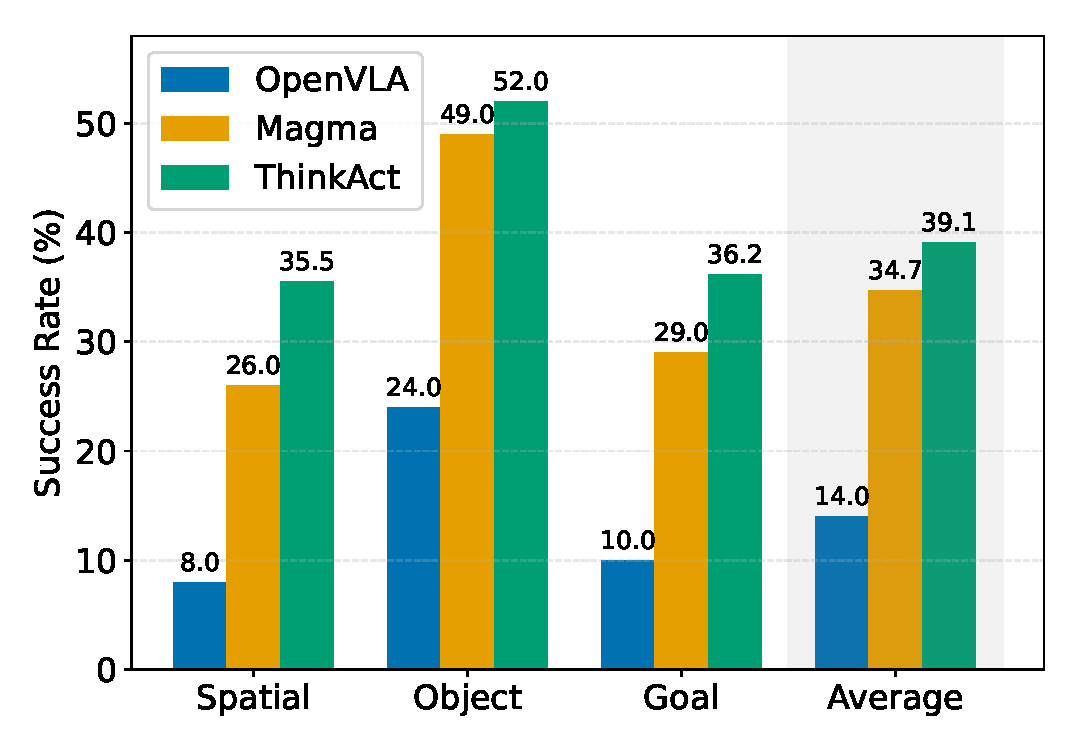
\includegraphics[width=\linewidth]{figures/images/fewshot.pdf}
        \vspace{-7mm}
        \caption{Few-shot adaptation results on LIBERO. We use 10 demonstrations per task for fine-tuning.}
        \label{fig:fewshot}
    \end{minipage}%
\end{figure}